\chapter{System Analysis and Data Acquisition}
\label{chap:chapter2}

\section{Functional Analysis of the 3D Printer}

The BCN3D+ is a Cartesian fused deposition modeling (FDM) 3D printer with dual independent extruders. It runs Marlin 1.x firmware and is managed through OctoPrint \cite{octoprint2024api}. For the purpose of fault detection, the system can be divided into five key subsystems \cite{blanchard2011systems}.

The extruder assembly is the most failure-prone part of the printer. It includes the hotend (nozzle, heater block, and thermistor), the cold end (heatsink, heat break, and cooling fan), and the extruder drive system (stepper motor and drive gear). The main observable signals from this subsystem include nozzle temperature (actual versus target), heatsink temperature measured using a KY-013 sensor, vibration of the assembly captured by an MPU-6050 sensor, and extrusion state information obtained from OctoPrint. Filament movement is calculated via the simple mouse encoder.

The motion system follows a Cartesian X-Y-Z architecture. The X-axis moves the print head using a GT2 belt, the Y-axis moves the build platform, and the Z-axis is controlled by two lead screws. Observable signals include axis positions (X, Y, Z, and extrusion axis in millimeters), commanded feedrate, and tri-axis vibration measurements from an MPU-6050 mounted on the X-carriage \cite{mpu6050_datasheet}.

The heated bed subsystem is responsible for maintaining adhesion during the first layer of printing. Its main monitored signals are the actual and target bed temperatures.

The electronics and control board consist of a RAMPS 1.4 board with an ATmega2560 microcontroller running Marlin firmware \cite{marlin2024thermal}. Relevant observable signals include firmware-level events and communication reliability indicators such as resend counts.

The cooling system includes two fans: one for part cooling and one for heatsink cooling. Failure of the heatsink fan is particularly critical because it can lead to heat creep. This is monitored indirectly through the rate of increase in heatsink temperature over time.

OctoPrint serves as a non-invasive bridge between the printer firmware and external systems, exposing telemetry data through an MQTT interface \cite{mqtt5_spec}. Data collected from the system is stored using Python-based collectors in two SQLite databases: \texttt{printer\_data.db}, which contains firmware telemetry, and \texttt{sensor\_data.db}, which stores external sensor measurements \cite{sqlite2024}.

Table~\ref{tab:printer_data_schema} presents the database schema for \texttt{printer\_data.db}. The table is organised by logical groups: \texttt{temperatures} (nozzle actual/target, bed, chamber), \texttt{motion} (axis positions, extruder position, feedrate), \texttt{print\_job} (filename, state, progress, filament used), \texttt{printer\_state} (printing/paused/error flags), \texttt{events} (firmware events for ground truth), and \texttt{resends} (communication reliability indicators).

\begin{table}[H]
\centering
%\caption{Database schema for \texttt{printer\_data.db}}
% ============================================================
% TABLE: Database schema for printer_data.db
% ============================================================
\scriptsize
\rowcolors{2}{white}{primary!10}
\begin{xltabular}{\linewidth}{| L{2.5cm} | L{2.5cm} | X |}
\caption{Database schema for \texttt{printer\_data.db}}
\label{tab:printer_data_schema} \\
\hline
\rowcolor{primary}
\textbf{\color{white}Table} & \textbf{\color{white}Column} & \textbf{\color{white}Description / Purpose} \\
\hline
\endfirsthead

\caption[]{Database schema for \texttt{printer\_data.db} (\textit{continued})} \\
\hline
\rowcolor{primary}
\textbf{\color{white}Table} & \textbf{\color{white}Column} & \textbf{\color{white}Description / Purpose} \\
\hline
\endhead

\hline
\multicolumn{3}{r}{\textit{Continued on next page\ldots}} \\
\endfoot

\hline
\endlastfoot

% --- temperatures table
temperatures & nozzle\_actual\_tool0 / tool1 & Actual nozzle temperature (°C) per extruder; primary thermal fault signal \\
\hline
temperatures & nozzle\_target\_tool0 / tool1 & Target setpoint; used to compute nozzle\_error = actual – target (heat creep, clog detection) \\
\hline
temperatures & bed\_actual\_c / bed\_target\_c & Heated bed temperature; bed adhesion fault detection \\
\hline
temperatures & chamber\_actual\_c & Enclosure ambient temperature; environmental context for thermal drift \\
\hline

% --- motion table
motion & x\_mm / y\_mm / z\_mm & Current axis positions in mm; kinematic synchronisation with 3D DT model \\
\hline
motion & e\_mm & Extruder position (cumulative filament pushed); extrusion/retraction state detection \\
\hline
motion & feedrate\_mmmin & Current commanded feedrate; used in vibration\_per\_feedrate cross‑feature \\
\hline

% --- print_job table
print\_job & filename / state & Active print file name and state (printing, paused, etc.); session context \\
\hline
print\_job & progress\_pct / elapsed\_s & Print progress percentage and elapsed time; temporal context for anomaly trending \\
\hline
print\_job & filament\_used\_mm & Cumulative filament consumed; material waste tracking \\
\hline

% --- printer_state table
printer\_state & printing / paused / error & Boolean flags (0/1); gate for fault detection logic (only alert during active printing) \\
\hline

% --- events table
events & event\_name / details\_json & OctoPrint firmware events (errors, warnings); labelled ground truth for ML training \\
\hline

% --- resends table
resends & resend\_count / ratio & G‑code retransmission count and ratio; indicator of communication reliability / step loss \\
\hline

\end{xltabular}
\label{tab:printer_data_schema}
\end{table}

\section{Failure Mode and Effects Analysis (FMEA)}

Failure Mode and Effects Analysis (FMEA) is used to systematically identify potential failure modes, their causes and effects, and to prioritize them using the Risk Priority Number (RPN), defined as Severity × Occurrence × Detection. This method is widely used in reliability engineering to guide maintenance and monitoring strategies \cite{liu2013risk, iec60812}.

Table~\ref{tab:fmea} presents the FMEA worksheet for the BCN3D+ printer. Six failure modes are identified as highest priority: nozzle clogging (RPN 392), overheating (RPN 180), misalignment/layer shifting (RPN 210), bearing wear (RPN 210), step loss (RPN 210), and belt breakage (RPN 168). For each failure mode, the table lists the affected subsystem, failure cause, observable effect, and the Severity, Occurrence, and Detection scores used to compute the RPN.

\begin{table}[H]
\centering
%\caption{FMEA worksheet for BCN3D+ FDM printer}
% ============================================================
% TABLE: FMEA worksheet (longtable)
% ============================================================
{
\scriptsize
\rowcolors{2}{white}{primary!10}
\begin{xltabular}{\linewidth}{| J | J | J | J | c | c | c | c | c |}
	\caption{FMEA worksheet for BCN3D+ FDM printer}
	\label{tab:fmea} \\
	\hline
	\rowcolor{primary}
	\textbf{\color{white}Failure Mode} & \textbf{\color{white}Subsystem} & \textbf{\color{white}Failure Cause} & \textbf{\color{white}Failure Effect} & \textbf{\color{white}S} & \textbf{\color{white}O} & \textbf{\color{white}D} & \textbf{\color{white}RPN} & \textbf{\color{white}Priority} \\
	\hline
	\endfirsthead

	\hline
	\rowcolor{primary}
	\textbf{\color{white}Failure Mode} & \textbf{\color{white}Subsystem} & \textbf{\color{white}Failure Cause} & \textbf{\color{white}Failure Effect} & \textbf{\color{white}S} & \textbf{\color{white}O} & \textbf{\color{white}D} & \textbf{\color{white}RPN} & \textbf{\color{white}Priority} \\
	\hline
	\endhead

	\hline
	\multicolumn{9}{r}{\textit{Continued on next page\ldots}} \\
	\endfoot

	\hline
	\endlastfoot

	Nozzle clogging & Extruder & Filament impurities, carbonised residue, heat creep & Under-extrusion, print cessation, material waste & 8 & 7 & 7 & 392 & CRITICAL \\
	\hline
	Overheating (thermal runaway) & Extruder / Bed & Heater cartridge failure, PID instability, fan failure & Component damage, fire risk, print failure & 9 & 4 & 5 & 180 & HIGH \\
	\hline
	Misalignment (layer shifting) & Motion system & Belt slippage, loose pulley, acceleration too high & Dimensional inaccuracy, failed print & 7 & 5 & 6 & 210 & HIGH \\
	\hline
	Bearing wear & Motion / Extruder & Lubrication loss, prolonged use, dust contamination & Vibration increase, positional error, seizure & 6 & 5 & 7 & 210 & HIGH \\
	\hline
	Step loss (missed steps) & Motion / Electronics & Driver overheating, current too low, mechanical obstruction & Layer offset, print failure, position error & 7 & 6 & 5 & 210 & HIGH \\
	\hline
	Belt breakage & Motion system & Fatigue, improper tensioning, foreign objects & Complete motion failure, immediate print loss & 8 & 3 & 7 & 168 & MEDIUM \\
	\hline
\end{xltabular}
}
\label{tab:fmea}
\end{table}

Nozzle clogging is the highest priority failure mode (RPN 392) and can be detected through vibration anomalies captured by the MPU-6050, low filament flow using our filament encoder and abnormal temperature increases at the heatsink measured by the KY-013 sensor. Overheating (RPN 180) and layer shifting (RPN 210) are also high-priority issues. Bearing wear and step loss (both RPN 210) can be identified through long-term trends in vibration RMS values and increases in communication resend counts \cite{randall2011vibration}. Belt breakage (RPN 168) is typically not detected at the exact moment of failure but instead through early degradation patterns such as vibration changes and motion inconsistencies.

\section{Sensor Selection}

Sensor selection is guided by three main criteria: the ability to observe relevant failure modes, feasibility of installation without modifying the printer firmware, and a strict hardware cost limit of under 50 euros \cite{shomenov2025}.

Table~\ref{tab:sensor_selection} summarises the sensors selected for the prototype. For each sensor, the table reports the measured parameter, target failure modes, physical placement on the printer, sampling rate, and implementation details. The selected sensors include the KY-013 NTC thermistor (heatsink temperature), MPU-6050 IMU (3-axis acceleration and gyroscope), OctoPrint MQTT telemetry (position, feedrate, temperatures), and an optical mouse-based filament encoder.

{% 
    \centering
    % ============================================================
% TABLE: Sensor selection summary (longtable)
% ============================================================
\rowcolors{2}{white}{primary!10}
\begin{longtable}{|P{2.2cm}|P{2.4cm}|P{2.4cm}|P{2.2cm}|P{1.8cm}|P{2.8cm}|}
    \caption{Sensor selection summary for BCN3D+ digital twin prototype}
    \label{tab:sensor_selection} \\

	\hline
	\rowcolor{primary}
	\textbf{\color{white}Sensor / Module} & \textbf{\color{white}Measured Parameter} & \textbf{\color{white}Target Failure Mode} & \textbf{\color{white}Physical Placement} & \textbf{\color{white}Sampling Rate} & \textbf{\color{white}Implementation} \\
	\hline
	\endfirsthead

	\hline
	\rowcolor{primary}
	\textbf{\color{white}Sensor / Module} & \textbf{\color{white}Measured Parameter} & \textbf{\color{white}Target Failure Mode} & \textbf{\color{white}Physical Placement} & \textbf{\color{white}Sampling Rate} & \textbf{\color{white}Implementation} \\
	\hline
	\endhead

	\hline
	\multicolumn{6}{r}{\textit{Continued on next page\ldots}} \\
	\endfoot

	\hline
	\endlastfoot

	KY-013 (NTC Thermistor) & Contact temperature (\textdegree{}C) & Nozzle clogging, overheating, heat creep & Extruder heatsink (primary); heated bed (secondary) & 2 Hz & ESP8266 ADC, Steinhart-Hart conversion; $R_{\mathrm{ref}} = 10\,\mathrm{k}\Omega$ \\
	\hline
	MPU-6050 / GY-521 (MEMS IMU) & 3-axis acceleration + gyroscope & Nozzle clogging (vibration spike), bearing wear, step loss, belt resonance & X-axis carriage, adjacent extruder nozzle & 50 Hz & I\textsuperscript{2}C to ESP8266; raw ADC integers $\rightarrow$ feature engineering (RMS, kurtosis, crest factor) \\
	\hline
	OctoPrint MQTT telemetry & Position (X, Y, Z, E mm), feedrate, nozzle/bed temperature setpoints and actuals, print state, filament used & Step loss, misalignment, overheating (via setpoint deviation) & Software bridge, no additional hardware & $\sim$1--5 Hz (polling interval) & OctoPrint MQTT plugin; JSON payloads to Mosquitto broker on Raspberry Pi \\
	\hline
	Position / end-stop sensors & Limit switch state (triggered / free) & Step loss, misalignment (homing failure) & X-min, Y-min, Z-min positions & Event-driven & Firmware-native; exposed via OctoPrint API, no additional hardware required \\
	\hline
	Camera (optional --- USB / Pi Camera) & Frame images of print surface & Layer delamination, warping, geometric defects & Fixed position above build plate, facing print surface & 1--5 fps & Not included in v1 baseline, reserved for future vision-based Tier 3 (DL) extension \\
	\hline
	Filament encoder (optical mouse) & 1-axis filament movement (mm/s) & Nozzle clogging, irregular filament flow, filament runout & Between filament spool and extruder motor & 1--5 Hz & Custom driver manipulation and manual calibration of raw optical sensor data \\
	\hline
\end{longtable}
    \label{tab:sensor_selection}
}

The KY-013 NTC thermistor measures heatsink temperature at 2 Hz using Steinhart-Hart conversion \cite{steinhart1968calibration}. It provides an accuracy of approximately ±1.6°C and enables early detection of heat creep through the rate of temperature increase.

The MPU-6050 MEMS inertial measurement unit provides six-axis acceleration and gyroscope data. It is mounted on the X-carriage and sampled at 50 Hz. Sensitivity has been validated in the 18--116 Hz range \cite{kiran2022sensitivity}. From this sensor, features such as RMS, kurtosis, crest factor, and FFT-based spectral energy are extracted for anomaly detection \cite{randall2011vibration}.

Additional sensors such as current sensing (ACS712) and vision-based monitoring are excluded from the current implementation due to budget constraints and non-invasive design requirements \cite{obico2024}. These are reserved for future system extensions.

The filament mouse encoder measures filament flow from the spool to the extruder at 1-5 Hz, enables early clog detection by comparing set and calculated feedrate speeds in a time window.

\section{Data Acquisition and Communication}

The system architecture follows an edge computing approach, where all processing is performed locally on a Raspberry Pi gateway \cite{shi2016edge}.

An ESP8266 microcontroller is used to sample the MPU-6050 at 50 Hz and the KY-013 at 2 Hz \cite{esp8266_trm}. It computes basic signal deltas and publishes structured JSON messages via MQTT. Telemetry data is transmitted using QoS 0, while critical alerts use QoS 1 \cite{mqtt5_spec}.

A Mosquitto MQTT broker runs on the Raspberry Pi and manages communication topics including \texttt{printer/sensors}, \texttt{printer/octoprint/\#}, and \texttt{printer/alerts/\#}.

The OctoPrint REST API is used both to retrieve the initial printer state and to send control commands such as pausing a print job when critical anomalies are detected \cite{octoprint2024api}.

Figure~\ref{fig:dfd} presents the Data Flow Diagram (DFD) of the acquisition pipeline. The diagram shows the flow of data from the physical printer and external sensors through the ESP8266 node and OctoPrint, into the MQTT broker, then to the Python collectors, SQLite databases, data aligner, feature engineering module, and finally to the PMx AI pipeline and dashboard.

\begin{figure}[H]
    \centering
    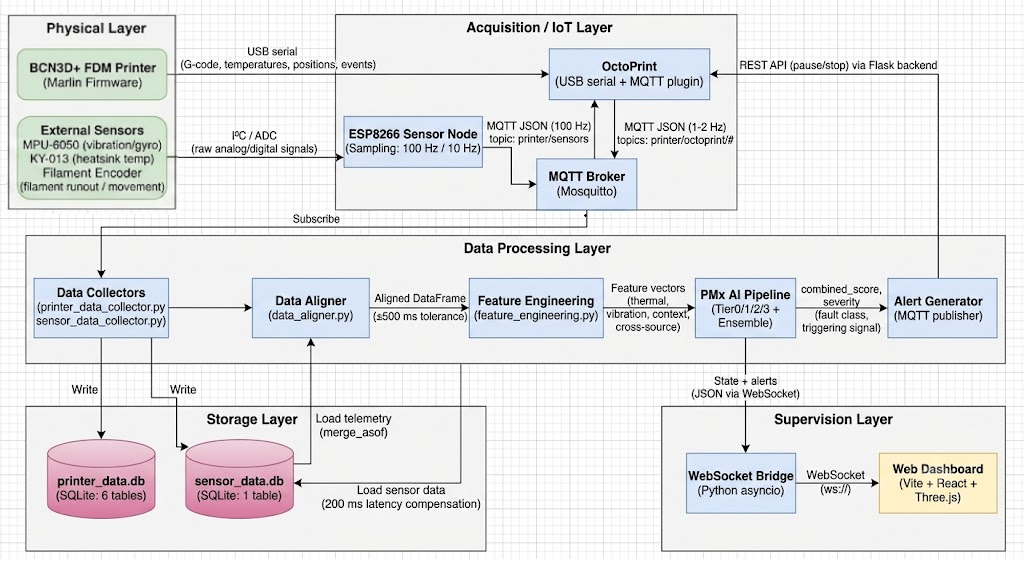
\includegraphics[width=0.9\textwidth]{figures/diagram_data_flow}
    %\caption{Data Flow Diagram (DFD) of the acquisition pipeline}
    \label{fig:dfd}
\end{figure}

As illustrated in the accompanying system architecture diagram, this acquisition process is part of a broader, five-tier pipeline:

\begin{itemize}
    \item \textbf{Physical \& Acquisition Layers:} Raw data from the BCN3D+ printer and external sensors flows into the ESP8266 node and OctoPrint, which then publish to the centralized Mosquitto MQTT broker.
    
    \item \textbf{Data Processing \& Storage Layers:} Subscribed data is written to local SQLite databases (\texttt{printer\_data.db} and \texttt{sensor\_data.db}). This telemetry is subsequently loaded, aligned (with latency compensation), and passed through feature engineering before entering the PMx AI Pipeline.
    
    \item \textbf{Supervision Layer:} The AI pipeline outputs fault classes and severity scores, forwarding states and alerts via a WebSocket bridge to a React/Three.js Web Dashboard. Simultaneously, the Alert Generator closes the loop by pushing critical pause/stop commands back to OctoPrint via its REST API.
\end{itemize}

The system relies on these two SQLite databases to handle the incoming telemetry. Table~\ref{tab:sensor_data_schema} describes the columns of \texttt{sensor\_data.db}, which stores external sensor readings. The table includes timestamp information (UTC and elapsed milliseconds), temperature readings (raw and delta), tri-axis accelerometer and gyroscope data (raw and delta), source identifier, and extrusion speed.

{%
    \centering
    % ============================================================
% TABLE: Database schema for sensor_data.db
% ============================================================
\scriptsize
\rowcolors{2}{white}{primary!10}
\begin{xltabular}{\linewidth}{| L{3.5cm} | L{3.0cm} | X |}
\caption{Database schema for \texttt{sensor\_data.db}}
\label{tab:sensor_data_schema} \\
\hline
\rowcolor{primary}
\textbf{\color{white}Column} & \textbf{\color{white}Type} & \textbf{\color{white}Description / Purpose} \\
\hline
\endfirsthead

\caption[]{Database schema for \texttt{sensor\_data.db} (\textit{continued})} \\
\hline
\rowcolor{primary}
\textbf{\color{white}Column} & \textbf{\color{white}Type} & \textbf{\color{white}Description / Purpose} \\
\hline
\endhead

\hline
\multicolumn{3}{r}{\textit{Continued on next page\ldots}} \\
\endfoot

\hline
\endlastfoot

timestamp\_utc & TEXT & ISO 8601 with milliseconds; primary join key for merge\_asof alignment with printer\_data.db \\
\hline
elapsed\_ms & INTEGER & Milliseconds since sensor node boot; used to detect sensor restarts \\
\hline
temp\_c & REAL & Converted Celsius temperature from KY-013 NTC thermistor via Steinhart-Hart equation \\
\hline
delta\_temp\_c & REAL & Temperature change since last sample; rate-of-rise detection (heat creep early warning) \\
\hline
acc\_x / acc\_y / acc\_z & INTEGER & Raw ADC counts from MPU-6050 accelerometer; 3-axis vibration data \\
\hline
delta\_acc\_x / delta\_acc\_y / delta\_acc\_z & INTEGER & Sample-to-sample acceleration delta; used in kurtosis and crest factor computation \\
\hline
gyro\_x / gyro\_y / gyro\_z & INTEGER & Raw ADC counts from MPU-6050 gyroscope; rotational dynamics (belt resonance, axis jerk) \\
\hline
delta\_gyro\_x / delta\_gyro\_y / delta\_gyro\_z & INTEGER & Gyroscope rate-of-change; complementary to acceleration for motion fault detection \\
\hline
source & TEXT & Sensor node identifier; traceability for multi-node deployments \\
\hline
extrusion & FLOAT & Extrusion speed (mm/s), used to describe the flow state of the filament relative to the configured feed rate \\
\hline

\end{xltabular}
    \label{tab:sensor_data_schema}
}


Time alignment between datasets is handled using Pandas \texttt{merge\_asof} with a 200 millisecond latency compensation and a ±500 millisecond tolerance window \cite{mckinney2010data}. A dedicated data alignment module shifts sensor timestamps backward by 200 milliseconds to compensate for MQTT transmission delay and then performs nearest-neighbor matching with OctoPrint telemetry.

The resulting synchronized dataset is used for feature engineering in the next chapter. Overall, this acquisition pipeline enables real-time, low-cost monitoring of the FDM printer without requiring any modification to the firmware, directly supporting the digital twin objectives introduced earlier.

\endinput